% slide and subtitle generation
    % latex beamer
    % latex compilation feedback (warnings) as visual inspector
% cursor generation
    % ROI by GUI instead of clip
% speech and talking-head generation
% parallel novelty compared with pixel level video gen

\vspace{-0.5\baselineskip} 
\section{\agent~Agent}
\vspace{-0.6\baselineskip} 
\textbf{Overview.} 
To address these challenges and liberate researchers from the burdensome task of manual video preparation, we introduce {\agent}, a multi-agent framework designed to automatically generate presentation videos directly from academic papers. 
As illustrated in Figure~\ref{fig:method}, to decouple the different roles, making the method scalable and flexible, the pipeline comprises four builders:
% \kevin{pdf /pptx I/O should be acceptable, here don't include quite a lot of details such as GUI / WhisperX}
\textbf{(i)} Slide builder. Given the paper, we first synthesize slides with \LaTeX~code and refine them with compilation feedback to correct grammar and optimize layout; 
%’s \LaTeX{} project (\textit{e.g.}, source code and figures)
\textbf{(ii)} Subtitle builder. The slides are then processed by a VLM to generate subtitles and sentence-level visual-focus prompts;  \textbf{(iii)} Cursor builder. These prompts are then grounded into on-screen cursor coordinates and synchronized with the narration.
% The finalized slides are then processed by a vision–language model (VLM) to produce a subtitle script and assign a visual-focus cue to each sentence. Then, a GUI model grounds every cue as a precise on-screen cursor trajectory, while WhisperX temporally aligns the cursor with the narration. 
\textbf{(iv)} Talker builder. Given the voice sample and the portrait of the speaker, text-to-speech and talking-head modules generate a realistic, personalized talker video. 
%For clarity, we denote $p,a,v$ for the slides, speech audio, and human presentation video, respectively, and $l,a_o,v_o$ for the input \LaTeX{} project, the speaker’s voice sample, and portrait.
For clarity, we denote the paper document, author portrait, and voice sample as $\mathcal{D}$, $\mathcal{I}$, and $\mathcal{A}$, respectively.


% \kevin{paper doc: $\mathcal{D}$, author image: $\mathcal{I}$, voice audio: $\mathcal{A}$}

% We propose {\agent} to address the identified challenges and enable automatic academic presentation video generation. The pipeline consists of three key components: \textbf{1. SlidePilot}: Takes the paper \LaTeX{} project as input and designs the slides by writing beamer code. Based on the compilation feedback, it fixes the error and introduces a visual-selection module to improve slide layouts. \textbf{2. TalkNavigator}: Generates the subtitle with cursor prompt  for each sentence to indicate visual anchors, and grounds cursor location by a GUI model and corresponding timesteps by WhishperX. \textbf{3. PresentCaptain}: Generates personalized speech with given voice sample and talking-head with presenter portrait. 

% Requires: \usepackage{algorithm,algpseudocode}

% Requires: \usepackage{algorithm,algpseudocode}




% Requires: \usepackage{algorithm,algpseudocode}

% \begin{algorithm}[b]
% \footnotesize
% \caption{Visual-Selective Layout Refinement}
% \label{alg:visual-selective}
% \begin{algorithmic}[1]
% \Require Compilable slide code $c^*$; text font scales $\mathcal{A}_{\text{text}}$; figure font scale $\alpha_{\text{fig}}$; figure scales $\mathcal{B}$
% \Ensure Refined slide code $c^{\dagger}$ and slides $s$
% \State $(\_, w)\gets\operatorname{Compile}(c^*)$;\ \ $\mathcal{I}\gets\operatorname{OverfullFrames}(w)$
% \If{$\mathcal{I}=\varnothing$} \State \Return $c^{\dagger}\gets c^*$ \EndIf
% \For{\textbf{each } $i\in\mathcal{I}$}
%   \State $s\gets\operatorname{ExtractFrame}(c^*,i)$;\ \ $\mathcal{C}\gets\varnothing$
%   \If{$\operatorname{IsTextOnly}(s)$}
%     \State $\mathcal{C}\gets\{\operatorname{ApplyFontScale}(s,\alpha):\alpha\in\mathcal{A}_{\text{text}}\}$
%   \Else \Comment{contains figures}
%     \State $s_{\text{font}}\gets\operatorname{ApplyFontScale}(s,\alpha_{\text{fig}})$ \Comment{shrink text once}
%     \State $\mathcal{C}\gets\{s_{\text{font}}\}\ \cup\ \{\operatorname{ApplyFigureScale}(s_{\text{font}},\beta):\beta\in\mathcal{B}\}$
%   \EndIf
%   \State $\text{img}\gets\{\operatorname{RenderAsImage}(c \text{ with } s' \text{ at } i): s'\in\mathcal{C}\}$
%   \State $s^{\star}\gets\arg\max_{s'\in\mathcal{C}}\ \operatorname{VLM\_Judge}(\text{img}[s'],\text{prompt}_{\text{layout}})$
%   \State $c\gets\operatorname{ReplaceFrame}(c,i,s^{\star})$
% \EndFor
% \State $c^{\dagger}\gets c$ \Comment{single refinement pass}
% \State \Return $s\gets\operatorname{CompilePDF}(c^{\dagger})$
% \end{algorithmic}
% \end{algorithm}



% 1. why we use latex--beamer, complete information, more coding-friendly
% \textbf{Key challenges -- how to effectively identify and debugging}
% , rendering
% from environment
% [fig.] prev. v.s. after (our visual-prompt)
% \noindent\textbf{Slide Generation.} 
% \kevin{One preliminary stage how human prepare the pre. video is create the slide, despite there have some existing works e.g., but we distingish them from}
\vspace{-0.4\baselineskip} 
\begin{figure}[t]
    \centering
    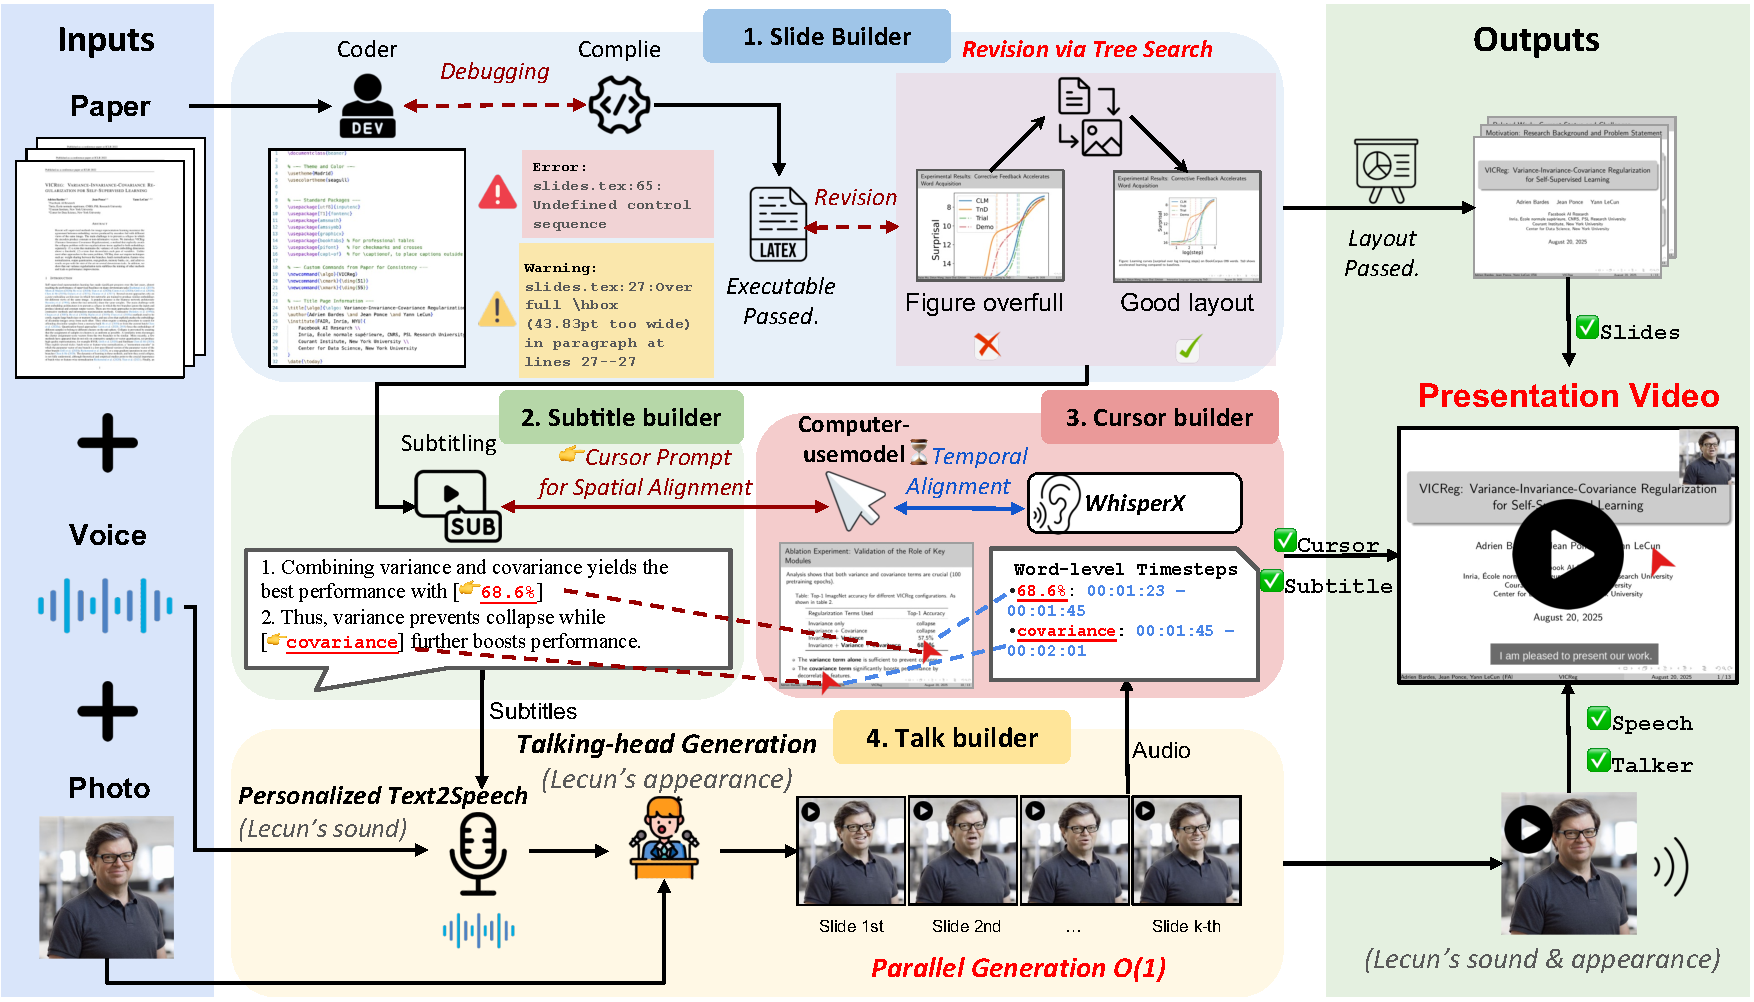
\includegraphics[width=\linewidth]{figure/method.pdf}
    \caption{\textbf{Overview of {\agent}.} Our pipeline comprises three key modules: \textbf{(i)} tree search visual choice for fine-grained slide layout optimization; \textbf{(ii)} a GUI-grounded model paired with WhisperX for spatiotemporally aligned cursor grounding; and \textbf{(iii)} slide-wise parallel generation for efficiency.}
    \label{fig:method}
\end{figure}

\subsection{Slide Builder}
\vspace{-0.4\baselineskip}
% \kevin{accept $\mathcal{D}$, output $\mathcal{S}$, $\mathcal{S}_0$ per page}
A prerequisite for producing a presentation video is the creation of the slides. Despite there being some existing works~\cite{zheng2025pptagent}, we target the generation of academic slides with fine-grained layouts and formal structure from scratch.
% \textbf{Why we use Latex \& Beamer}
Rather than selecting a template and iteratively editing it with VLMs, we generate slides directly from a paper’s \LaTeX{} project by prompting the model to write Beamer code. We adopt Beamer for three reasons: \textbf{(i)} \LaTeX{}’s declarative typesetting automatically arranges text block and figures from their parameters without explicitly planing the positions; \textbf{(ii)} Beamer is compact and expressive, representing the same content in fewer lines than XML-based formats; and \textbf{(iii)} Beamer provides well-designed, formally configured styles (\textit{e.g.}, page numbers, section headers, hyperlinks) that are well suited to academic slide design.

% As \(l=(t,\mathcal{F})\) denote the project of paper, where \(t\) is the text source code and \(\mathcal{F}=\{f_i\}_{i=1}^{n}\) are the figure paths.
Given the paper $\mathcal{D}$ as input, the LLM first produces a draft slide code. We compile this code to collect diagnostics(\ie~errors and warnings). Then, we use the error information to elicit a repaired correct code.
% , as shown in Alogrithm~\ref{alg:compile-repair}
This procedure ensures that the generated Beamer code is grammatically correct and effectively leverages and faithfully covers its content.
% , yielding the content of slides that are ready to use.

Although \LaTeX{} can automatically arrange the location of the contents in the slides, the generated slides could sometimes still suffer from inappropriate layouts (\textit{e.g.}, overflow) due to the unsuitable parameters for figure or text font size. However, as the compilation warning signals potential layout issues, we are able to first use them to identify the slides that require refinement.
% \kevin{One challenging is that LLm fail to preceive visually, thus} 
% as LLM fail to perceive visual feedback like human designers,
\begin{wrapfigure}[18]{r}{0.4\textwidth} % 12=大致占用的行数,可调 8~16
  %\vspace{-0.5\baselineskip}              % 往上顶,避免与上一行留白
  \centering
  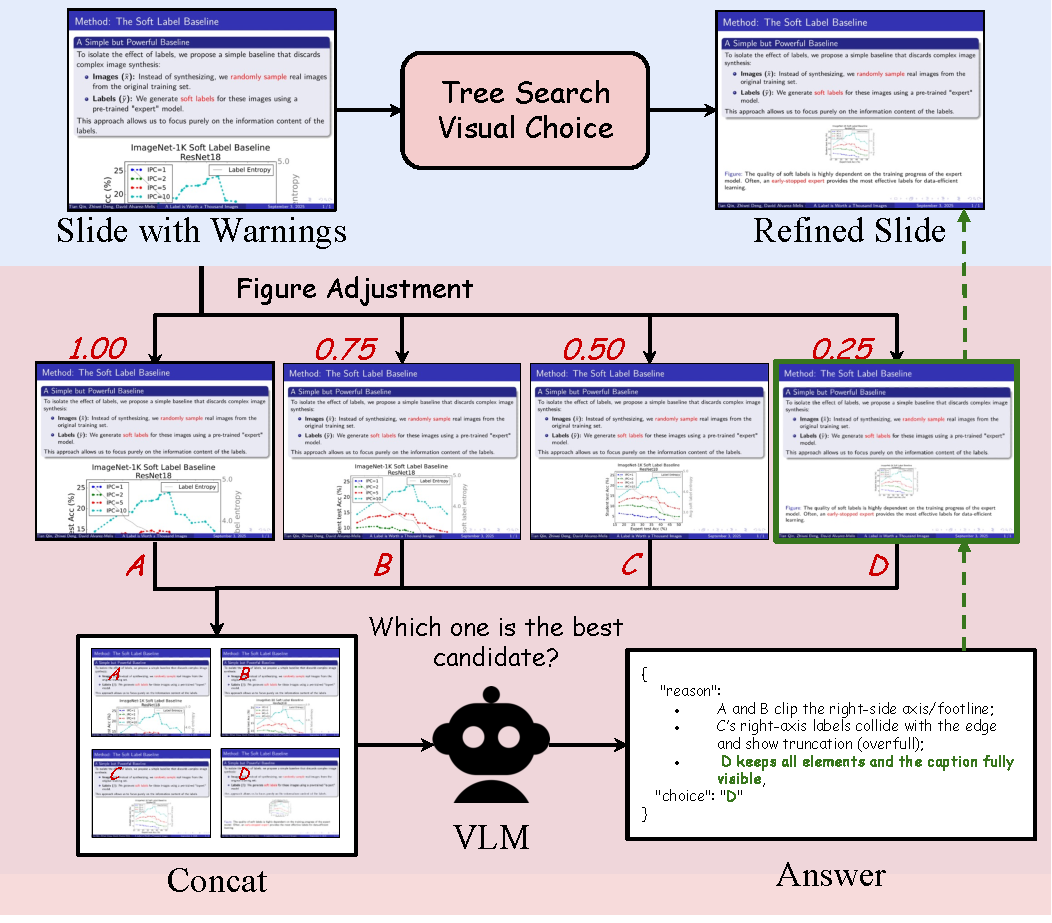
\includegraphics[width=\linewidth]{figure/tree_search.pdf}
  \captionsetup{skip=2pt}                 % 图↔标题更紧
  \caption{\textbf{Tree Search Visual Choice.} It combines a rule-based proposal mechanism with VLM-based scoring to select the optimal candidate.}
  \label{fig:mcts}
  %\vspace{-1\baselineskip}              % 与后续正文再贴近
\end{wrapfigure}

\vspace{-1\baselineskip}
\noindent\textbf{Tree Search Visual Choice.} After localizing the slides that require refinement, the key challenge is how to adjust their layouts effectively. As LLMs/VLMs fail to perceive real-time visual feedback like human designers, we observe that prompting the them to directly tune numeric layout parameters (\textit{e.g.}, font sizes, margins, figure scales) is ineffective: the models are largely \textbf{insensitive} to small numeric changes, yielding unstable and inefficient refinement, consistent with limitations of the parameter-editing strategy in PPTAgent~\cite{zheng2025pptagent}. To address this limitation, we introduce a \emph{visual-selection} module for overflowed slides. The module first constructs the neighborhoods of layout variants for the current slide by rule-based adjusting the figure and text parameters, renders each variant to an image, and then uses the VLMs as a judge to score the candidates and select the one with the best layout. Specifically, for text-only slides, we sweep the font size; for slides with figures, we first vary the figure scaling factors (\textit{e.g.}, 1.25, 0.75, 0.5, 0.25) and then reduce the font size, details shown in Figure~\ref{fig:mcts}. These edits are straightforward in \LaTeX{} Beamer, whose structured syntax automatically reflows content as parameter changes. This module \textbf{decouples discrete layout search from semantic reasoning} and reliably resolves overflow cases with minimal time and tokens.

After fixing the errors and adjusting the parameters, we compile the slide code to obtain the finalized slides $\mathcal{S}_i,i=1,\dots,n$ with fine-grained layouts, where $n$ indicates the number of slides.
% \kevin{wondering add a small fig here. add a figure}

% \textbf{decompose, modular}
% either pdf input / latex input are both available;

% non-trivial
% \begin{wrapfigure}[12]{r}{0.5\textwidth} % 12=大致占用的行数,可调 8~16
%   %\vspace{-0.5\baselineskip}              % 往上顶,避免与上一行留白
%   \centering
%   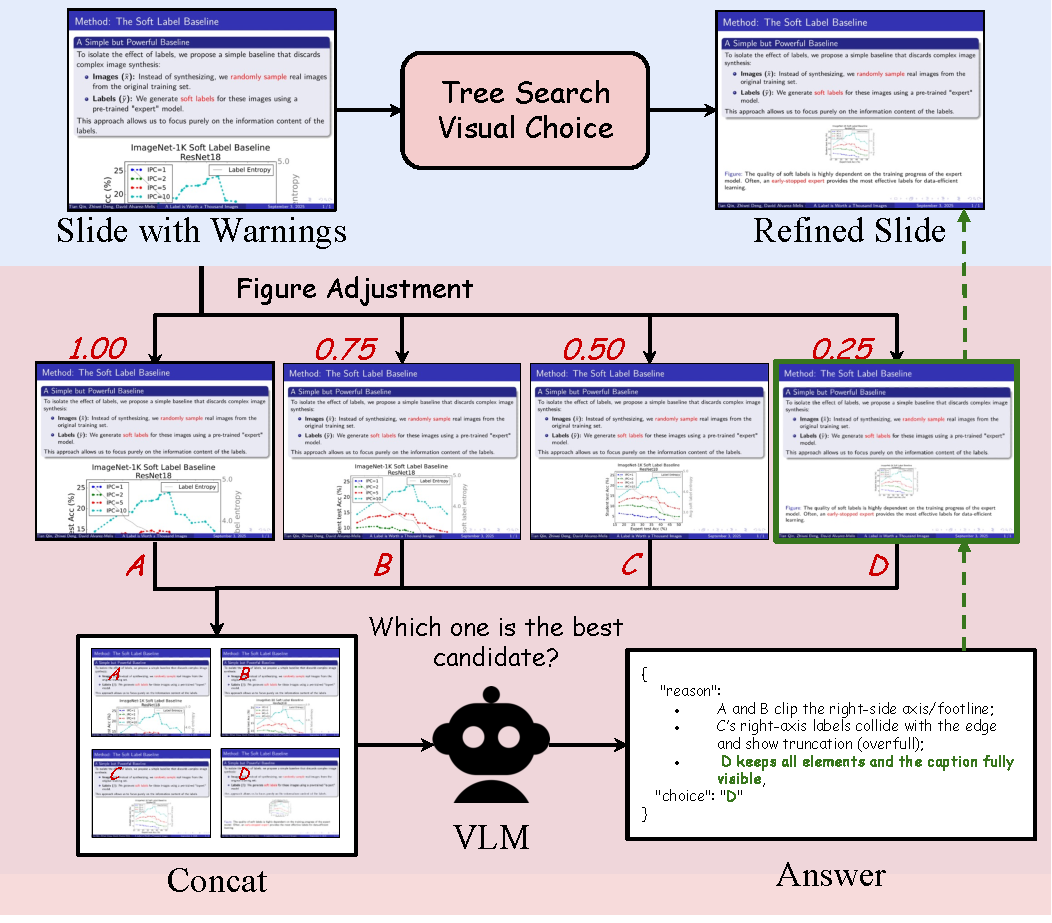
\includegraphics[width=\linewidth]{figure/tree_search.pdf}
%   \captionsetup{skip=2pt}                 % 图↔标题更紧
%   \caption{\textbf{Tree Search Visual Choice.} It combines a rule-based proposal mechanism with VLM-based scoring to select the optimal candidate.}
%   \label{fig:mcts}
%   %\vspace{-1\baselineskip}              % 与后续正文再贴近
% \end{wrapfigure}

\vspace{-0.4\baselineskip} 
\subsection{Subtitle Builder}
\vspace{-0.4\baselineskip} 
% \kevin{$\mathcal{S}_0$ slide, output a transcript $\mathcal{T}_0$, cursor prompt $\mathcal{P}_{0}^i$}
% \kevin{what's the challenging here, are we apply the parallel gen here also? why slide in rather than paper in? because less context; why create visual-focus from subtitle? usually, when human talking some slide with sentence, they have some focusness on keywords; \textbf{inputs, outputs}}
As the speech should follow the slides, given the generated slide $\mathcal{S}_i$, we rasterize them into images and pass them to a VLM, which produces sentence-level subtitles $T_{i}^{j}$ and its corresponding visual-focus prompt $P_{i}^{j}$. The visual-focus prompt serves as an intermediate representation linking speech to the cursor, enabling precise temporal and spatial alignment of the cursor with the narration in order to improve audience guidance, which will be discussed in Section~\ref{sec:cursor}.

\vspace{-0.5\baselineskip} 
\subsection{Talker Builder}
\vspace{-0.5\baselineskip} 
% consider formal, gesture, thus we choose which models (digital)
% \textbf{Key challenges -- bottlenect of cascade generation long video}
% 5min, per slide very slow;
% [highlight insights from real huamn recording]
% usually / practically, gen per page independent, so this motivate us to develop a parallel strategy,
% \kevin{$\mathcal{T}$, $\mathcal{A}$, $\widetilde{\mathcal{A}}$, $\mathcal{V}_0$}
The presenter video is vital for audience engagement and conveying the researcher’s scholarly identity (\textit{e.g.}, face and voice). Given the subtitles $\mathcal{T}_i$, the author’s portrait $\mathcal{I}$, and a short voice sample $\mathcal{A}$, our objective is to synthesize a presenter video that delivers the slide content in the author’s voice, with faithful identity preservation and lip–audio synchronization.

\vspace{-0.4\baselineskip}
\noindent\textbf{Subtitle-to-Speech.} Given subtitles and voice sample, we use F5-TTS~\cite{tts-f5} to generate speech audio per slide, \begingroup \small $
\widetilde{\mathcal{A}}_i = \operatorname{TTS}\!\left( \{\, T_{i}^{j} \,\}_{j=1}^{m_i} |\mathcal{A}\right), i=1,\ldots,n, $
\endgroup ~where $m_i$ is the number of the sentences in $\mathcal{T}_i$.

\vspace{-0.4\baselineskip}
\noindent\textbf{Parallel Talkinghead Generation.} 
% \kevin{add intuition here, in real-world human also prepare videos like this} 
To balance fidelity and efficiency, we use Hallo2~\cite{cui2024hallo2} for head-only synthesis and employ FantasyTalking~\cite{fantasytalking} to support talking generation with upper-body articulation.
%considering its higher computational cost. 
A persistent challenge is the long generation time: generating only a few minutes of talking-head video typically takes several hours, and some models(\textit{e.g.}, FantasyTalking) do not yet natively support long-video generation. 
% To alleviate this bottleneck, 
Inspired by the common practice of slide-by-slide recording and the independence between each slide, we synthesize the presenter video on a per-slide basis. Specifically, for each slide $\mathcal{S}_i$, given the audio condition $\widetilde{\mathcal{A}}_i$ and portrait $\mathcal{I}$, we generate an independent clip $\mathcal{V}_i$ and execute these jobs in parallel, markedly reducing generation time: \begingroup \small $\mathcal{V}_i = \mathcal{G}\!\left(\widetilde{\mathcal{A}}_i, \mathcal{I}\right), i=1,\ldots,n,$\endgroup ~where $\mathcal{G}$ represents the talking-head generation model.
This design is justified because slide transitions are hard scene changes, and the temporal continuity of the presenter across adjacent slides is unnecessary.

\vspace{-0.5\baselineskip} 
\subsection{Cursor Builder}
\vspace{-0.5\baselineskip} 
\label{sec:cursor}
% \textbf{Key challenges -- How to associate / map speech improtance with visually}
% usually, the speaker will have keywords in each sentence, so parse keyword, then, motivated by strong Computer-use model, this can be a query XX
% [fig.] how speech sentence -> keyword -> computer use [x,y] -> screenshot
\textbf{Spatial-Temporal Grounding.}
% \kevin{input $\mathcal{P}_{0}^i$ with a slide $\mathcal{S}_0$, then output a coordinate $[x,y]$}
% \kevin{For spatial: we are motivated by Computer-ues grounding, which simulates user interaction xxx}
In practice, presenters leverage the cursor as an attentional guide: a well-aligned cursor trajectory minimizes extraneous cognitive load, helps the audience track the presentation, and keeps focus on the key content. However, automatic cursor-trajectory grounding is nontrivial, requiring simultaneous alignment to the timing of speech and the visual semantics of the slides. To simplify the task, we assume that the cursor will stay still within a sentence and only move between the sentences. Thus, we estimate a per-sentence cursor location and time span. For spatial alignment, motivated by strong computer-use models~\cite{lin2025showui,qin2025ui} which simulate user interaction with the screenshot, we propose to ground the cursor location $(x,y)$ for each sentence with the visual focus prompt $\mathcal{P}_{i}^{j}$ by UI-TARS~\cite{qin2025ui}. To achieve precise temporal alignment, we then use WhisperX~\cite{bain2023whisperx} to extract word-level timestamps and align them with the corresponding sentence in the subtitles to derive the start and end times $(t_s,t_e)$ of each cursor segment.
% \kevin{For temporal: we aim to get precise alignment, while sentence is not satisfy, thus we use world-alignment}
